%! Author = csefalvayk
%! Date = 7/11/21
\documentclass{article}
\usepackage[T1]{fontenc}
\usepackage[p,osf]{cochineal}
\usepackage{setspace}
\usepackage[scale=.95,type1]{cabin}
\usepackage[cochineal,bigdelims,cmintegrals,vvarbb]{newtxmath}
\usepackage[zerostyle=c,scaled=.94]{newtxtt}
\usepackage[cal=boondoxo]{mathalfa}
\usepackage{amsfonts}
\usepackage{url}
\usepackage[table,xcdraw]{xcolor}
\usepackage{booktabs}
\usepackage{multirow}
\usepackage{tikz}
\usetikzlibrary{shapes,arrows}
\usepackage{caption}
\usepackage{float}
\newcommand*{\h}{\hspace{5pt}}% for indentation
\newcommand*{\hh}{\h\h}% double indentation


% Bibliography styling
\usepackage[super,square,sort&compress,numbers]{natbib}
\bibliographystyle{unsrtnat}
\usepackage{graphicx}
\usepackage{hyperref}

\title{Anaphylactic events in mRNA vaccines: a case-control reporting study}

% Authors, for the paper (add full first names)
\author{Chris von Csefalvay\thanks{Starschema Inc., Arlington, VA. Correspondence: \texttt{csefalvayk@starschema.net}.}}

\begin{document}

\maketitle

\onehalfspacing

\begin{abstract}
    TBD.
\end{abstract}

\section{Introduction}

\subsection{Background}

Anaphylaxis describes a severe systemic allergic reaction to an antigen, resulting in large-scale mast cell degranulation and, consequently, histamine release.\cite{metcalfe2009mechanisms}
In clinical practice, it typically manifests as an acute onset of respiratory symptoms, bronchoconstriction, urticaria, flushing, gastrointestinal symptoms (nausea, vomiting, diarrhoea) and reduced blood pressure.\cite{lee2011anaphylaxis}
Anaphylactic reactions to vaccines, while fortunately vanishingly rare, are well-documented in relation to a wide range of vaccines.\cite{su2019anaphylaxis,kelso1999anaphylaxis,kelso1993anaphylaxis,nagao2016highly}
The COVID-19 vaccines approved in the United States (BNT162b2/tozinameran, commonly known as the Pfizer/BioNTech vaccine, and mRNA-1273/elasomeran, commonly known as the Moderna vaccine) are no exceptions in this regard.
Rare episodes of anaphylaxis have been documented in the context of both the Moderna\cite{covid2021allergicmoderna} and the Pfizer/BioNTech vaccine.\cite{shimabukuro2021allergic}

Because of the severity and, absent rapid and appropriate medical intervention, life-threatening nature of anaphylactic reactions, severe allergic adverse events have been key drivers behind vaccine hesitancy.\cite{tulloch2021covid,marcec2021postvaccination,jacobson2015vaccine}
Since the Pfizer/BioNTech and Moderna vaccines represent the first prophylactic mRNA based vaccines in wider public health use, understanding the true risk of anaphylaxis from these vaccines is crucial to address vaccine hesitancy and safeguard the goals of the COVID-19 vaccination programmes worldwide.

\subsection{Objectives}\label{subsec:objectives}

The objective of this study was threefold:

\begin{enumerate}
    \item to investigate the effect of mRNA vaccination versus a non-mRNA vaccination on the likelihood of reporting an anaphylactic symptom to VAERS as opposed to a non-anaphylactic symptom,
    \item to quantify whether this effect is homogenous across strata of age group and gender, and
    \item to identify whether certain self-reported allergies are associated with a higher likelihood of reporting an anaphylactic symptom to VAERS as opposed to a non-anaphylactic symptom.
\end{enumerate}

It was hypothesised at the outset that the mRNA-based vaccines would not be associated with a statistically significant elevated odds ratio ($OR > 3.0$ at $p < 0.05$) in the whole-population samples.
In addition, we hypothesised with respect to the breakdown by gender that while women would be slightly more likely to present with anaphylactic events due to the higher prevalence of anaphylaxis in women in general,\cite{salvati2019gender} the relative difference as measured by Breslow-Day statistics of contingency tables stratified by gender would not be statistically significant.
We further hypothesised that age would also not play a significant role.
It was expected that relative homogeneity and Cochran-Mantel-Haenszel statistics of age-stratified contingency tables would confirm a pooled odds ratio quite close to unity and a relatively high degree of homogeneity between age band strata.


\section{Methods}

\subsection{Study design}

A case-control study, adhering to the STROBE Statement's methodology and best practices,\cite{von2014strengthening} was performed on reports to VAERS received between 01 January 2000 and 02 July 2021.
Reports were excluded if they did not name a specific vaccine type (VAERS parameter \texttt{VAX\_TYPE} of \texttt{UNK}), or if they pertained to an unidentified COVID-19 vaccine (VAERS parameter \texttt{VAX\_NAME} of \texttt{COVID19 (COVID19 (UNKNOWN))}).
Cases of anaphylaxis were identified by the VAERS symptom description, and mRNA vaccines by the name of the specific vaccine in respect of which the report was made.
These were matched against controls from the same subset of VAERS reports that reported non-anaphylactic reactions, with matching by age (rounded to the nearest integer) and reported gender.

\begin{figure}
    \centering
    \begin{center}
  \sffamily
  \footnotesize
  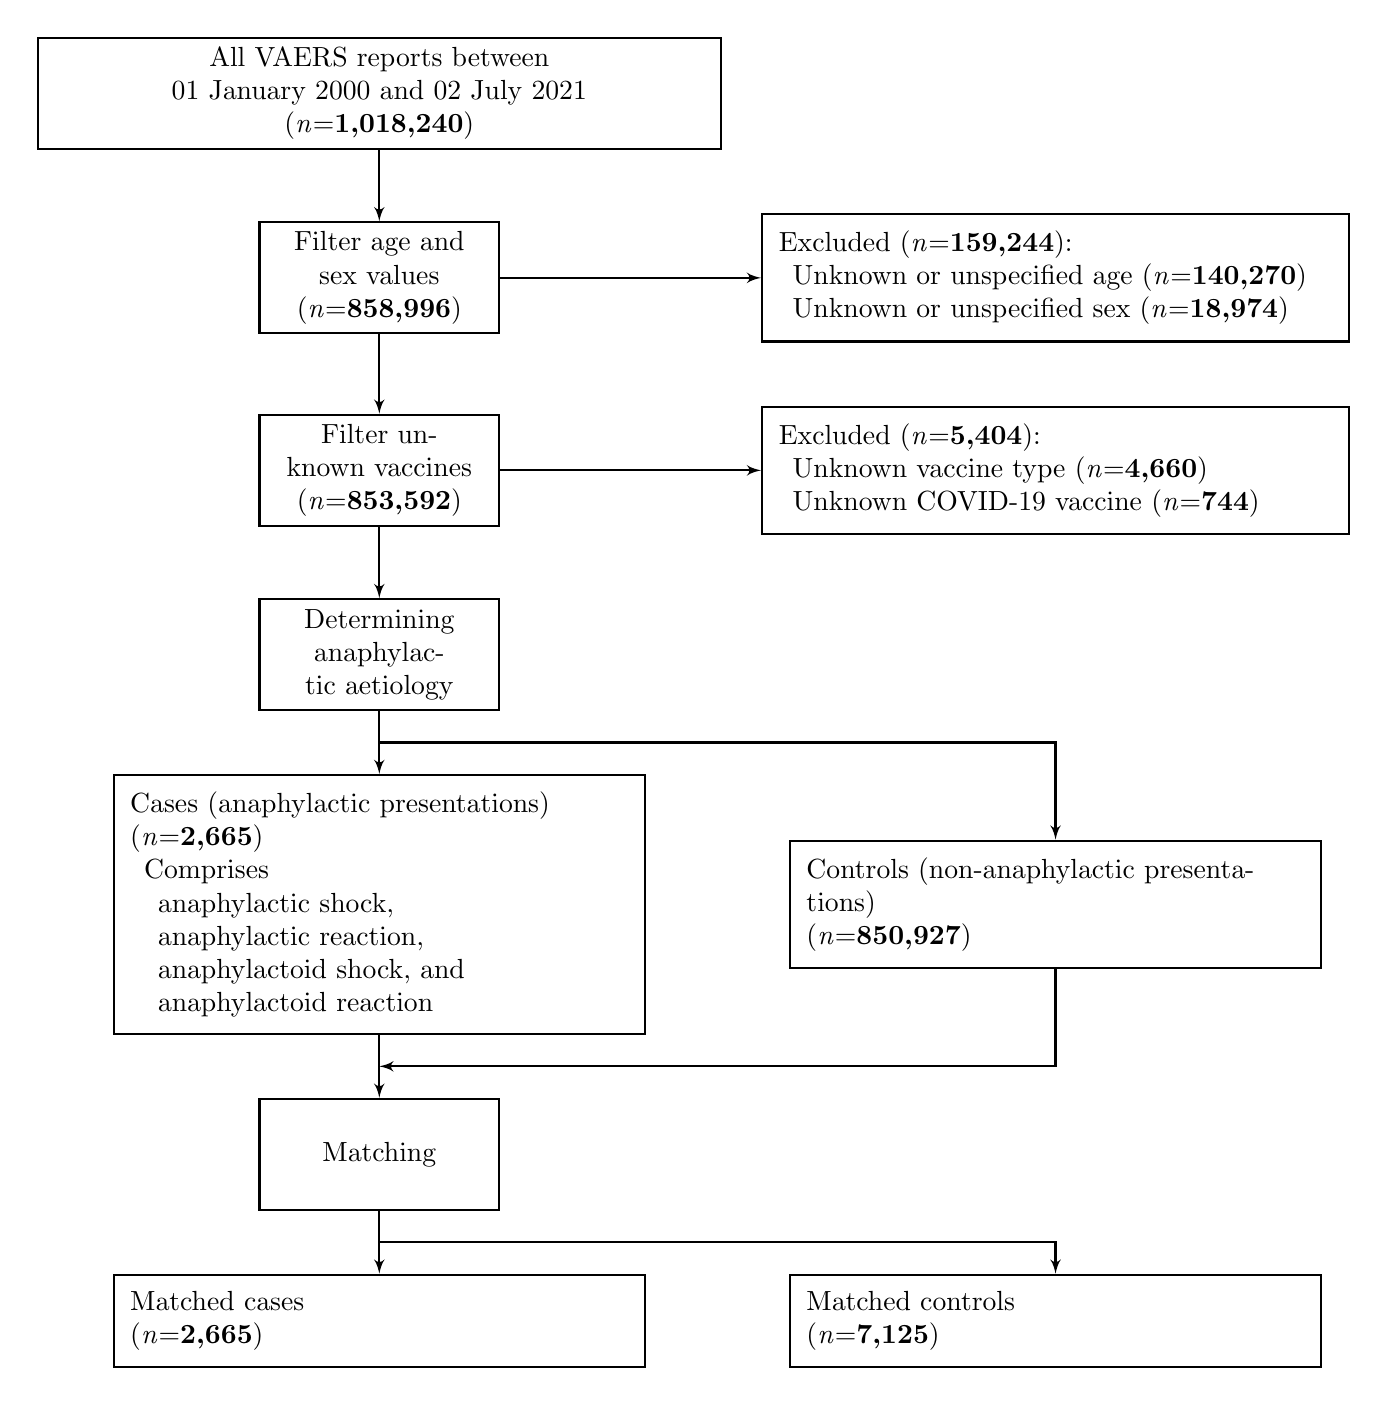
\begin{tikzpicture}[auto,
    %decision/.style={diamond, draw=black, thick, fill=white,
    %text width=8em, text badly centered,
    %inner sep=1pt, font=\sffamily\small},
    block_center/.style ={rectangle, draw=black, thick, fill=white,
      text width=8em, text centered,
      minimum height=4em},
    block_source/.style ={rectangle, draw=black, thick, fill=white,
      text width=24em, text centered,
      minimum height=4em},
    block_left/.style ={rectangle, draw=black, thick, fill=white,
      text width=20em, text ragged, minimum height=4em, inner sep=6pt},
    block_noborder/.style ={rectangle, draw=none, thick, fill=none,
      text width=18em, text centered, minimum height=1em},
    block_assign/.style ={rectangle, draw=black, thick, fill=white,
      text width=18em, text ragged, minimum height=3em, inner sep=6pt},
    block_lost/.style ={rectangle, draw=black, thick, fill=white,
      text width=16em, text ragged, minimum height=3em, inner sep=6pt},
      line/.style ={draw, thick, -latex'}]
    % outlining the flowchart using the PGF/TikZ matrix funtion
    \matrix [column sep=5mm,row sep=8mm] {
      % row 1
      \node [block_source] (loaded_vaers) {All VAERS reports between\\01 January 2000 and 02 July 2021\\(\textit{n}=\textbf{1,018,240})}; \\
      \node [block_center] (filter_age_sex) {Filter age and sex values (\textit{n}=\textbf{858,996})};
      & \node [block_left] (exclude_age_sex) {Excluded (\textit{n}=\textbf{159,244}):\\
                  \h Unknown or unspecified age (\textit{n}=\textbf{140,270})\\
                  \h Unknown or unspecified sex (\textit{n}=\textbf{18,974})}; \\
      \node [block_center] (filter_unknown_vax) {Filter unknown vaccines (\textit{n}=\textbf{853,592})};
      & \node [block_left] (exclude_unknown_vax) {Excluded (\textit{n}=\textbf{5,404}):\\
                  \h Unknown vaccine type (\textit{n}=\textbf{4,660})\\
                  \h Unknown COVID-19 vaccine (\textit{n}=\textbf{744})};\\
      \node [block_center] (anaphylaxis) {Determining anaphylactic aetiology}; \\
      \node [block_assign] (cases) {Cases (anaphylactic presentations)\\(\textit{n}=\textbf{2,665})\\
                  \h Comprises \\
                    \hh anaphylactic shock,\\
                    \hh anaphylactic reaction,\\
                    \hh anaphylactoid shock, and\\
                    \hh anaphylactoid reaction};
      & \node [block_assign] (controls) {Controls (non-anaphylactic presentations)\\(\textit{n}=\textbf{850,927})}; \\
      \node [block_center] (matching) {Matching}; \\
      \node [block_assign] (matched_cases) {Matched cases\\(\textit{n}=\textbf{2,665})};
      & \node [block_assign] (matched_controls) {Matched controls\\(\textit{n}=\textbf{7,125})}; \\
    };% end matrix
    % connecting nodes with paths
    \begin{scope}[every path/.style=line]
      \path (loaded_vaers)   -- (filter_age_sex);
      \path (filter_age_sex)   -- (filter_unknown_vax);
      \path (filter_age_sex)   -- (exclude_age_sex);
      \path (filter_unknown_vax)  -- (exclude_unknown_vax);
      \path (filter_unknown_vax)   -- (anaphylaxis);
      \path (anaphylaxis)  -- (cases) coordinate [midway](phoney1);
      \path (phoney1)  -| (controls);
      \path (cases)  -- (matching) coordinate [midway](phoney2);
      \path (matching)  -- (matched_cases) coordinate [midway](phoney3);
      \path (controls)  |- (phoney2);
      \path (phoney3)  -| (matched_controls);
    \end{scope}
  \end{tikzpicture}
\end{center}
    \caption{Patient disposition flow chart.}
    \label{fig:patient_disposition}
\end{figure}

Comparative statistical analyses were then utilised to determine statistical associations of risk.
In particular, stratified odds ratios were calculated for both the crude and the age- and gender-matched sets of reports by gender, age band and reported pre-existing hypersensitivities.
Cochran-Mantel-Haenszel statistics were used to determine pooled reporting odds ratios by strata, while inter-strata homogeneity was tested using the Breslow-Day metric.

\subsection{Data sources}

Data on adverse events following immunisations was obtained from VAERS via \url{vaers.hhs.gov} on 12 July 2021.
The data files from 2000 onwards were loaded and processed using Python 3.7.5 (Python Software Foundation, Fredericksburg, VA) and version 1.3.0 of the \texttt{pandas} package.\cite{mckinney2011pandas}
Ingested raw data thus included reports received by VAERS between 01 January 2000 and 02 July 2021.
Altogether, 1,018,240 reports were ingested in respect of the period under examination.

Of these, we have excluded 140,270 reports for a failure to state a valid age and 18,974 reports for specifying no or unknown biological sex.
In addition, 4,660 reports were excluded for disclosing an unknown vaccine type (\texttt{VAX\_TYPE} VAERS attribute of value \texttt{UNK}) and 744 reports were excluded for documenting the administration of an unknown COVID-19 vaccine (\texttt{VAX\_NAME} VAERS attribute of \texttt{COVID19 (COVID19 (UNKNOWN))}).
Following these exclusions, 853,592 eligible reports were processed.

A flow chart of this process is presented as Figure~\ref{fig:patient_disposition}.

\subsection{Identifying cases}\label{subsec:identifying-cases}

Cases were defined as reports to VAERS that reported one of four anaphylactic conditions.
These were selected from the Preferred Terms (PTs) that are classified by the MedDRA High Level Term (HLT) of Anaphylactic and anaphylactoid responses (MedDRA ID 10077535), under the explicit exclusion of three PTs that have no relevance for vaccine administration: dialysis membrane reactions (MedDRA ID 10076665), anaphylactic transfusion reactions (MedDRA ID 10067113) and anaphylactoid syndrome of pregnancy (MedDRA ID 10067010).
The ontology of the included diagnostic categories is presented in Table~\ref{tab:meddra-inclusion-ontology}.

\begin{table}[H]
\centering
\resizebox{\textwidth}{!}{%
\begin{tabular}{@{}llll@{}}
\toprule
\multicolumn{1}{c}{\textbf{SOC}} &
  \multicolumn{1}{c}{\textbf{HLGT}} &
  \multicolumn{1}{c}{\textbf{HLT}} &
  \multicolumn{1}{c}{\textbf{PT}} \\ \midrule
\multirow{7}{*}{\begin{tabular}[c]{@{}l@{}}Immune system disorders\\ 10021428\end{tabular}} &
  \multirow{7}{*}{\begin{tabular}[c]{@{}l@{}}Allergic conditions\\ 10001708\end{tabular}} &
  \multirow{7}{*}{\begin{tabular}[c]{@{}l@{}}Anaphylactic and\\ anaphylactoid\\ responses\\ 10077535\end{tabular}} &
  \textbf{\begin{tabular}[c]{@{}l@{}}Anaphylactic reaction\\ 10002198\end{tabular}} \\ \cmidrule(l){4-4}
 &
   &
   &
  \textbf{\begin{tabular}[c]{@{}l@{}}Anaphylactic shock\\ 10002199\end{tabular}} \\ \cmidrule(l){4-4}
 &
   &
   &
  \textbf{\begin{tabular}[c]{@{}l@{}}Anaphylactoid reaction\\ 10002216\end{tabular}} \\ \cmidrule(l){4-4}
 &
   &
   &
  \textbf{\begin{tabular}[c]{@{}l@{}}Anaphylactoid shock\\ 10063119\end{tabular}} \\ \cmidrule(l){4-4}
 &
   &
   &
  \begin{tabular}[c]{@{}l@{}}Dialysis membrane reaction\\ 10076665\end{tabular} \\ \cmidrule(l){4-4}
 &
   &
   &
  \begin{tabular}[c]{@{}l@{}}Anaphylactic transfusion reaction\\ 10067113\end{tabular} \\ \cmidrule(l){4-4}
 &
   &
   &
  \begin{tabular}[c]{@{}l@{}}Anaphylactoid syndrome\\ of pregnancy\\ 10067010\end{tabular} \\ \bottomrule
\end{tabular}%
}
\caption{MedDRA ontology of included diagnostic categories.
Preferred Terms that are considered an anaphylactic reaction are set in bold type.}
\label{tab:meddra-inclusion-ontology}
\end{table}

While MedDRA offers a Standardised MedDRA Query (SMQ) corresponding to anaphylaxis, this includes a wide range of clinical entities.
Some would introduce unnecessary confounders (such as hereditary anaphylactic disorders like C1 esterase deficiency), while others would lay the analysis open to clearly unconnected events (such as transfusion related anaphylactic events).
For this reason, we chose to construe anaphylaxis narrowly.
This yielded 2,665 cases of anaphylactic or anaphylactoid symptoms.

\subsection{Identifying controls}

We defined the possible pool of controls as any eligible reports that did not disclose an anaphylactic presentation.
850,927 eligible reports constituted the pool of potential controls.

\subsection{Identifying exposure}

Exposure was defined as the receipt of an mRNA vaccine, regardless of the order of administration.
A report was deemed to pertain to an mRNA vaccine if the vaccine administered had a \texttt{VAX\_NAME} VAERS attribute of

\begin{itemize}
    \item \texttt{COVID19 (COVID19 (MODERNA))} (elasomeran), or
    \item \texttt{COVID19 (COVID19 (PFIZER-BIONTECH))} (tozinameran).
\end{itemize}

\subsection{Case-control matching}

In order to reduce the confounding impacts of biological sex (due to the greater propensity of women to develop anaphylactic presentations) and age (due to the unusual age profile of the COVID-19 vaccinated demographic owing to the focus of early vaccination campaigns on the elderly and vulnerable), matching was performed over age (rounded to the nearest integer) and biological sex.
Matching was performed over the exact age, even if age banding is used later for stratification, so as to avoid 'edge effects' where inhomogenous distributions of cases within a stratum, peaking towards one or both of the margins, create additional confounding.
Separability was relatively weak but present at 55.51\% accuracy over 100 balanced models, suggesting that the benefits of matching might be modest but perceptible.
The 2,665 cases were matched to 7,125 controls using the propensity matching functionality of \texttt{pymatch}.
This gives an overall case:control ratio of 2.673 controls per case.

At an assumed 40\% exposure rate among controls, a power of 0.95 at a 95\% two-sided confidence level for an odds ratio at or above 1.5 would require between 437 and 453 cases and 1,168 to 1,211 controls, depending on whether Kelsey's or Fleiss's corrected method is used.\cite{kelsey1996methods,fleiss2013statistical}
At almost six times the required value, this case-control ratio gives a fairly high predictive power for odds ratios at least as extreme as 1.5.
The characteristics of the cases and the controls after matching are presented in Table~\ref{tab:case-control-characteristics}.

\begin{table}[]
\centering
\resizebox{\textwidth}{!}{%
\begin{tabular}{@{}lll@{}}
\toprule
 & \begin{tabular}[c]{@{}l@{}}Cases\\ (n = 2,665)\end{tabular} & \begin{tabular}[c]{@{}l@{}}Controls\\ (n = 7,125)\end{tabular} \\ \midrule
Sex                   &                    &                    \\
\rowcolor[HTML]{EFEFEF}
Male                  & 732 (28\%)         & 1,788 (25\%)       \\
\rowcolor[HTML]{C0C0C0}
Female                & 1,933 (72\%)       & 5,337 (75\%)       \\
Age group             &                    &                    \\
\rowcolor[HTML]{EFEFEF}
\textless{}18         & 596 (22\%)         & 1549 (22\%)        \\
\rowcolor[HTML]{C0C0C0}
19-25                 & 185 (7\%)          & 448 (6\%)          \\
\rowcolor[HTML]{EFEFEF}
26-35                 & 368 (14\%)         & 924 (13\%)         \\
\rowcolor[HTML]{C0C0C0}
36-45                 & 483 (18\%)         & 1,267 (18\%)       \\
\rowcolor[HTML]{EFEFEF}
46-55                 & 433 (16\%)         & 1,147 (16\%)       \\
\rowcolor[HTML]{C0C0C0}
56-65                 & 326 (12\%)         & 955 (13\%)         \\
\rowcolor[HTML]{EFEFEF}
66-75                 & 196 (7\%)          & 538 (8\%)          \\
\rowcolor[HTML]{C0C0C0}
76-85                 & 68 (3\%)           & 231 (3\%)          \\
\rowcolor[HTML]{EFEFEF}
86-95                 & 7 (\textless{}1\%) & 61 (1\%)           \\
\rowcolor[HTML]{C0C0C0}
\textgreater{}95      & 0 (0\%)            & 3 (\textless{}1\%) \\ \midrule
mRNA vaccine exposure &                    &                    \\
\rowcolor[HTML]{EFEFEF}
Yes                   & 1,352 (51\%)       & 3,116 (56\%)       \\
\rowcolor[HTML]{C0C0C0}
No                    & 1,313 (49\%)       & 4,009 (44\%)
\end{tabular}%
}
\caption{Descriptive statistics and exposure data of cases and controls.}
\label{tab:case-control-characteristics}
\end{table}

\subsection{Statistical analysis}

For the purposes of stratification (but not matching), ages were divided into age bands, with a separate age band for persons under the age of 18, 18-25 and thereafter in ten-year increments until the age of 95.
A residual age band for persons aged 96 and above was constructed. Following this segmentation, the analysis proceeded in three stages.

First, crude odds ratios were calculated for the entire sample before matching, along with pooled odds ratios by biological sex and age band.
For the analysis of stratified contingency tables, the Breslow-Day statistics were used to test for the homogeneity of odds ratios and the Cochran-Mantel-Haenszel test was used to arrive at a pooled odds ratio.
Statistical analysis used the \texttt{StratifiedTable} class of \texttt{statsmodels} 0.12.2.\cite{seabold2010statsmodels}

In the second stage, the same odds ratios were calculated, using the same stratification, over the age- and gender-matched sample.
This step, too, utilised Breslow-Day statistics for homogeneity \textit{inter strata} and the Cochran-Mantel-Haenszel test for calculating the pooled odds ratio.
In addition, odds ratios by stratum were calculated and Fisher's exact test was performed to identify the statistical significance of odds ratios by stratum.

Finally, odds ratios were calculated specifically for previous allergies.
Using regular expressions, the \texttt{ALLERGIES} field of each VAERS entry was examined for 17 individual classes of allergens.
Since this is a free text field, regular expressions had to be designed to capture most common ways of referring to a class of drugs or prominent instances thereof.
The list below reproduces, in parentheses, exemplary items that would respond to the class's defining regular expressions.

\begin{itemize}
    \item Opioids (e.g. \texttt{CDN}, \texttt{Oxycontin}, \texttt{pentazocine})
    \item Latex (e.g. \texttt{Latex})
    \item Macrolide and aminoglycoside antibiotics (e.g. \texttt{azithromycin}, \texttt{Z-pack})
    \item Tetracycline antibiotics (e.g. \texttt{tigecycline}, \texttt{doxycycline})
    \item Sulfas (e.g. \texttt{Bactrim}, \texttt{sulfonamides})
    \item Beta-lactam antibiotics (e.g. \texttt{Augmentin}, \texttt{penicillin}, \texttt{cefazolin})
    \item Fluoroquinolone antibiotics (e.g. \texttt{Cipro}, \texttt{levofloxacin})
    \item Hydrochlorothiazide (e.g. \texttt{HCTZ}, \texttt{hydrochlorothiazide})
    \item Glycols (e.g. \texttt{PEG}, \texttt{propylene glycol})
    \item Local anaesthetics (e.g. \texttt{lidocaine})
    \item Known vaccine hypersensitivities (e.g. \texttt{Hepatitis vaccine}, \texttt{Prevnar})
    \item Fish and seafood (e.g. \texttt{mussels}, \texttt{crab}, \texttt{seafood})
    \item Insect stings (e.g. \texttt{bee venom}, \texttt{wasps}, \texttt{bee strings})
    \item Eggs (e.g. \texttt{egg whites}, \texttt{egg protein})
    \item NSAIDs (e.g. \texttt{Motrin}, \texttt{Aspirin}, \texttt{naproxen})
    \item Peanuts and tree nuts (e.g. \texttt{walnuts}, \texttt{peanuts})
\end{itemize}

For the statistical analysis of stated allergies, only entries with a valid entry in the \texttt{ALLERGY} field were considered, and no crude (unmatched) values were calculated.

\section{Results}

\subsection{Anaphylactic events and mRNA vaccination}

The reporting odds ratio (ROR) of anaphylactic events among mRNA vaccination versus other events and non-mRNA vaccines was 1.325 (95\% CI: 1.212 -- 1.448).
This result was statistically significant at $p < 0.001$.
This ROR is highly statistically significant, but quite close to unity, indicating the absence of a strong statistical association between anaphylactic events and mRNA vaccination.
Persons reporting an anaphylactic event are thus, as hypothesised (see Subsection~\ref{subsec:objectives}), not significantly more likely to have received an mRNA vaccine than a non-mRNA vaccine.

\subsection{Gender and anaphylaxis risk}

It was one of our initial hypotheses that the ROR of anaphylactic events after mRNA vaccines would be slightly higher for women due to the overall higher prevalence of anaphylaxis in female populations, but that such difference would not be highly statistically significant (see Subsection~\ref{subsec:objectives}]).
This is confirmed by the results of our analysis.

The ROR for female participants was slightly higher than for male participants, and unlike for the latter group, it was statistically significant.
The Breslow-Day test, significant at $p < 0.05$, indicates statistically significant homogeneity between gender strata.
The Cochran-Mantel-Haenszel statistic, significant at $p < 0.001$, indicates a high likelihood of a common ROR of unity.

Consequently, the data appears to strongly confirm that after matching, gender is not a factor of significant influence on the reported association between mRNA vaccines and reports of anaphylaxis.
This analysis thus does not evidence a statistically significant gender-dependent differential risk of anaphylaxis.

\subsection{Age and anaphylaxis risk}

\begin{figure}[H]
\centering
\includegraphics[width=12.5 cm]{forest_plot_of_anaphylaxis_by_age}
\caption{Forest plot of reporting odds ratio of anaphylactic reactions upon receipt of an mRNA vaccine by age band.}
\label{fig:age-forest-plot}
\end{figure}

The pooled odds ratio by age bands was 1.441 (95\% CI: 1.302 -- 1.593).
The Breslow-Day test, significant at $p < 0.005$, indicates that despite small inhomogeneities that derive from the characteristic age-dependent demographics of anaphylaxis,\cite{lee2011anaphylaxis} the recipient's age band also was not a statistically significant confounder after matching.
The Cochran-Mantel-Haenszel statistic, which was significant at $p < 0.001$, confirmed a common ROR of unity.

As Figure~\ref{fig:age-forest-plot} indicates, only five age bands (26 -- 35, 46 -- 55, 56 -- 65, 66 -- 76 and 76 -- 85) show statistically significant results.
In all of these cases, the reporting odds ratio is modestly above unity but below 2.0, the minimum value commonly agreed to be the lowest possible cut-off for signal generation.
Taken together, it appears from the data that the risk of anaphylactic reactions is not strongly associated with the recipient's age.
Consequently, no age-dependent safety signals vis-a-vis anaphylaxis emerge from this analysis, and mRNA vaccines are according to this data not statistically significantly less safe than non-mRNA vaccines, regardless of age group.

\subsection{Previous allergies and anaphylaxis risk}

Of the 17 classes of allergens isolated from the \texttt{ALLERGY} free text field, 14 (82.4\%) were detected in both the control and case groups.
Breslow-Day analysis indicated that the strata were not significantly homogenous ($p = 0.204$).
This is highly suggestive of significant differences among allergic predispositions and anaphylaxis in mRNA vaccines.

Of the 14 relevant categories of allergies, only two were statistically significant.
It is notable that these two were also the highest RORs, and the only RORs exceeding 2 (see Figure~\ref{fig:allergies-forest-plot}).
Pre-existing allergies to NSAIDs (ROR: 3.382, 95\% CI: 1.362 -- 8.399, $p < 0.01$) and fluoroquinolone antibiotics (ROR: 5.586, 95\% CI: 1.119 -- 27.900) are associated with higher RORs of anaphylactic reactions.
Notably, there is no statistically significant association between pre-existing reports of allergic events (of any severity) from other vaccines, which is in line with the fundamental biochemical and compositional differences between mRNA vaccines and non-mRNA vaccines.


\begin{figure}
\centering
\includegraphics[width=12.5 cm]{forest_plot_of_anaphylaxis_by_known_allergies}
\caption{Forest plot of reporting odds ratio of anaphylactic reactions upon receipt of an mRNA vaccine by reported prior allergic status.}
\label{fig:allergies-forest-plot}
\end{figure}


\section{Discussion}

\subsection{mRNA vaccines are not associated with a higher risk of anaphylaxis}

We hypothesised that mRNA-based vaccines do not have a specific anaphylactogenic property, i.e. that they are not associated with a statistically significant elevated odds ratio in the whole population.
The overall ROR after matching for age and gender confirms this



It was hypothesised at the outset that the mRNA-based vaccines would not be associated with a statistically significant elevated odds ratio ($OR > 3.0$ at $p < 0.05$) in the whole-population samples.
In addition, we hypothesised with respect to the breakdown by gender that while women would be slightly more likely to present with anaphylactic events due to the higher prevalence of anaphylaxis in women in general,\cite{salvati2019gender} the relative difference as measured by Breslow-Day statistics of contingency tables stratified by gender would not be statistically significant.
We further hypothesised that age would also not play a significant role.
It was expected that relative homogeneity and Cochran-Mantel-Haenszel statistics of age-stratified contingency tables would confirm a pooled odds ratio quite close to unity and a relatively high degree of homogeneity between age band strata.


\subsection{Limitations}

\section{Conclusion}

%%%%%%%%%%%%%%%%%%%%%%%%%%%%%%%%%%%%%%%%%%
\vspace{6pt}

\section*{Supplementary material}

Supplementary material S1, a CSV (comma-separated values) version of the data underlying Figure~, is available as part of DOI 10.5281/zenodo.XXXXX.

\section*{Funding}

This research was funded by Starschema Inc. under its intramural research funding programme.

\section*{Data availability}

VAERS reporting data is available from the CDC's website at \url{https://vaers.hhs.gov}.
All code and scripts supporting this manuscript are deposited at
\url{https://github.com/chrisvoncsefalvay/covid-19-vaccine-anaphylaxis} and are made available under the DOI 10.5281/zenodo.XXXXXX.

\section*{Conflicts of interest}

CvC is a consultant to a company that may be affected by the research reported in this paper.
The funders had no role in the design of the study;
in the collection, analysis, or interpretation of data;
in the writing of the manuscript, or in the decision to publish the~results.

\bibliography{bibliography}

\end{document}
